
\chapter{Theory}
\section{Modeling of cameras}

Since all cameras project a 3D scene onto a 2D plane, there will be information lost about the depth of the image. It is therefore not possible to calculate the exact placement of an object from a single picture, unless you have extra information about the objects in the picture. For this reason it is easy to create a projection in a 3D scene, but hard to create a scene from a projection. In addition to this, the amount of pixels and the field of view also affect the information and detail in the captured image. The most basic camera model is called the pinhole model, and is applicable for most cameras without high distortion lenses.

\subsection{pinhole projection} \label{sec:pinhole}
The pinhole model is based on the first camera, the Camera Obscura, made in 1568. It captures a scene by projecting straight light rays through a common focal point, and through a plane. The projection itself is made from where the light rays intersect the projection plane. The focal length, $f$, and the image plane size will then decide the field of view, $\theta_x$ and $\theta_y$, as shown in Figure~\ref{fig:pinhole}. 

\begin{figure}[!htb]
    \centering

    \tdplotsetmaincoords{80}{145}
    \begin{tikzpicture}[tdplot_main_coords, scale = 1.8]
    
        \tdplotsetrotatedcoords{0}{-90}{90}
        \draw[tdplot_rotated_coords, ->] (-0.7,0,0) -- (2,0,0) node[below right]{$X$};
        \draw[tdplot_rotated_coords, ->] (0,-0.5,0) -- (0,1,0) node[right]{$Y$};
        \draw[tdplot_rotated_coords, dashed] (0,0,-0.5) -- (0,0,9.2);
        \draw[tdplot_rotated_coords, ->] (0,0,9.2) -- (0,0,10) node[below]{$z,Z$};
        
        \pgfmathsetmacro{\rvec}{8}
        \pgfmathsetmacro{\imgradius}{3}
        \pgfmathsetmacro{\thetavec}{12}
        \pgfmathsetmacro{\phivec}{8}
        
        \coordinate (O) at (0,0,0);
        \tdplotsetcoord{P1}{\rvec}{90 -\phivec}{180 - \thetavec}
        \tdplotsetcoord{longP1}{\rvec*1.1}{90 -\phivec}{180 - \thetavec}
        \tdplotsetcoord{P2}{\rvec}{90 +\phivec}{180 - \thetavec}
        \tdplotsetcoord{longP2}{\rvec*1.1}{90 +\phivec}{180 - \thetavec}
        \tdplotsetcoord{P3}{\rvec}{90 + \phivec}{180 + \thetavec}
        \tdplotsetcoord{longP3}{\rvec*1.1}{90 +\phivec}{180 + \thetavec}
        \tdplotsetcoord{P4}{\rvec}{90 - \phivec}{180 + \thetavec}
        \tdplotsetcoord{longP4}{\rvec*1.1}{90 -\phivec}{180 + \thetavec}
        
        \tdplotsetcoord{IMG1}{\imgradius}{90 -\phivec}{180 - \thetavec}
        \tdplotsetcoord{IMG2}{\imgradius}{90 +\phivec}{180 - \thetavec}
        \tdplotsetcoord{IMG3}{\imgradius}{90 +\phivec}{180 + \thetavec}
        \tdplotsetcoord{IMG4}{\imgradius}{90 -\phivec}{180 + \thetavec}
        \coordinate (IMGC) at (-2.906,0,0);
        
        \shade[tdplot_rotated_coords, ball color=blue!50, opacity = 0.7] (0,0,8) circle (1cm); 

        \tdplotsetrotatedcoordsorigin{(IMGC)} %\imgradius*sin(90-\phivec)*cos(180-\thetavec)
        \shade[tdplot_rotated_coords, ball color=blue!50, opacity = 0.7] (0,0,0) circle (0.375);
        \draw[tdplot_rotated_coords, ->] (-0.7,0,0) -- (2,0,0) node[below right]{$x$};
        \draw[tdplot_rotated_coords, ->] (0,-0.5,0) -- (0,1,0) node[right]{$y$};
        
        \draw[] (IMG1) -- (IMG2) -- (IMG3) -- (IMG4) -- cycle;
      
        \draw[] (0,0,0.75) -- (0,0,0.85); \draw[] (0,0,0.8) -- (-2.906,0,0.8); \draw[] (-2.906,0,0.75) -- (-2.906,0,0.85);
        \draw[] (-1.45,0,1) node{$f$};
        
        \draw[thick, opacity = 0.3] (O) -- (P1); \draw[dashed, opacity = 0.3] (P1) -- (longP1);
        \draw[thick, opacity = 0.3] (O) -- (P2); \draw[dashed, opacity = 0.3] (P2) -- (longP2);
        \draw[thick, opacity = 0.3] (O) -- (P3); \draw[dashed, opacity = 0.3] (P3) -- (longP3);
        \draw[thick, opacity = 0.3] (O) -- (P4); \draw[dashed, opacity = 0.3] (P4) -- (longP4);
        
        \tdplotsetthetaplanecoords{180-\thetavec}
        \tdplotdrawarc[tdplot_rotated_coords]{(O)}{5}{90-\phivec}{90+\phivec}{anchor=west}{$\theta_y$}
        \tdplotsetrotatedcoords{0}{\phivec}{90}
        \tdplotdrawarc[tdplot_rotated_coords]{(O)}{5}{90-\thetavec}{90+\thetavec}{anchor=south}{$\theta_x$}
        
        
    \end{tikzpicture}

    \caption{Pinhole projection with the image plane between the focal point and the object}
    \label{fig:pinhole}
    
\end{figure}

Using the properties of similar triangles, the relationship between the World coordinates, $X,Y,Z$ and the image coordinates $x,y$ becomes:

\begin{align}
    tan(\phi_x) &= \frac{x}{f} = \frac{X}{Z} & tan(\phi_y) &= \frac{y}{f} = \frac{Y}{Z} \label{eq:pinhole_tan_relation} \\
    x &= f\frac{X}{Z} & y &=f\frac{Y}{Z}
    \label{eq:pinhole_relation}
\end{align}

As seen in Equation \eqref{eq:pinhole_relation}, the relationship between the sizes nonlinear. In order to present this in matrix form, the homogenous coordinates $p=[x,y,1]^\top$ and $P=[X,Y,Z,1]^\top$ are used. The matrix transformation is shown in Equation~\eqref{eq:pinhole_matrix}, with the imtermediate step $p^*$ being $p$ scaled by $Z$.

\begin{align}
    p^* &= \begin{bmatrix}
        x^* \\ y^* \\ z^*
    \end{bmatrix} = \begin{bmatrix}
        f & 0 & 0 & 0 \\
        0 & f & 0 & 0 \\
        0 & 0 & 1 & 0
    \end{bmatrix}\begin{bmatrix}
        X \\ Y \\ Z \\ 1
    \end{bmatrix} &
    p &= \frac{1}{z^*}p^*
    \label{eq:pinhole_matrix}
\end{align}

Since the light rays need to pass through the pinhole and onto the image plane, it is not possible to have a field of view larger than $180^\circ$. As seen in Equation~\eqref{eq:pinhole_matrix}, the projected object is also scaled by the distance to it, causing the points where the vertical field of view is $180^\circ$ to be singular. 

In a digital camera, the image plane consists of a small chip with a discrete amount of light sensitive elements, or pixels. Defining a new pixel coordinate frame to consist of the image pixels, with the origin in the upper left corner, as shown in Figure~\ref{fig:rel_img_pixel}. Using $W$ and $H$ as the image width and height in pixels, the transformation from image coordinates to pixel coordinates will be as shown in Equation~\eqref{eq:pixel_transform}.

\begin{figure}[!htb]
    \centering
    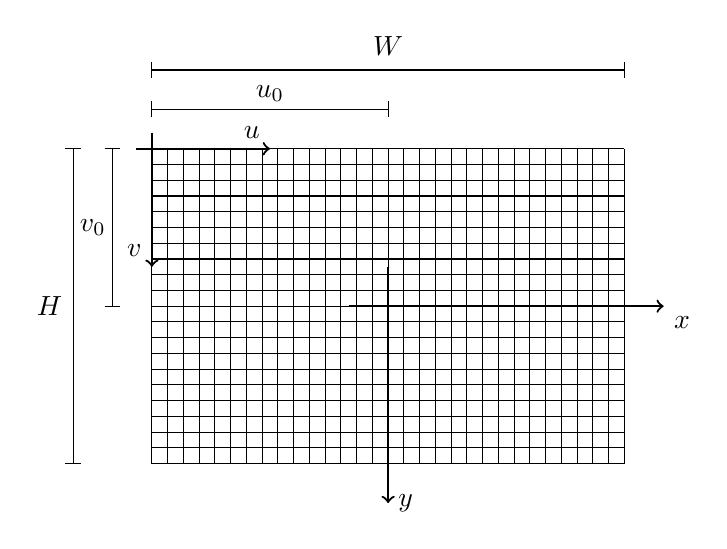
\begin{tikzpicture}[scale = 1.0]
    
    \draw[thick, ->] (-0.5,0,0) -- (3.5,0,0) node[below right]{$x$};
    \draw[thick, ->] (0,0.5,0) -- (0,-2.5,0) node[right]{$y$};
    \draw[thick, ->] (-3.2,2,0) -- (-1.5,2,0) node[above left]{$u$};
    \draw[thick, ->] (-3,2.2,0) -- (-3,0.5,0) node[above left]{$v$};
    
    \draw[] (-3,3,0) -- (3,3,0); \draw[] (-3,2.9,0) -- (-3,3.1,0); \draw[] (3,2.9,0) -- (3,3.1,0);
    \draw[] (-3,2.5,0) -- (0,2.5,0); \draw[] (-3,2.4,0) -- (-3,2.6,0); \draw[] (0,2.4,0) -- (0,2.6,0);
    \draw[] (-1.5,2.7,0) node{$u_0$};
    \draw[] (0,3.3,0) node{$W$};
    
    \draw[] (-4,2,0) -- (-4,-2,0); \draw[] (-4.1,2,0) -- (-3.9,2,0); \draw[] (-4.1,-2,0) -- (-3.9,-2,0);
    \draw[] (-3.5,2,0) -- (-3.5,0,0); \draw[] (-3.6,2,0) -- (-3.4,2,0); \draw[] (-3.6,0,0) -- (-3.4,0,0);
    \draw[] (-3.75,1,0) node{$v_0$};
    \draw[] (-4.3,0,0) node{$H$};
    
    \foreach \yline in {-2,-1.8,...,2} {
        \draw[] (-3, \yline, 0) -- (3, \yline, 0);
    } %end foreach
    
    \foreach \xline in {-3,-2.8,...,3} {
        \draw[] (\xline, -2, 0) -- (\xline, 2, 0);
    } %end foreach
    
    \end{tikzpicture}
    
    \caption{Relationship between pixel and image coordinates}
    \label{fig:rel_img_pixel}
\end{figure}

\begin{equation}
    p^i = \begin{bmatrix}
        u \\ v \\ 1
    \end{bmatrix} = \begin{bmatrix}
        \frac{W}{2x_{max}} & 0 & u_0 \\
        0 & \frac{H}{2y_{max}} & v_0 \\
        0 & 0 & 1
    \end{bmatrix}p =
    \begin{bmatrix}
        \frac{W}{2x_{max}} & 0 & u_0 \\
        0 & \frac{H}{2y_{max}} & v_0 \\
        0 & 0 & 1
    \end{bmatrix}\begin{bmatrix}
        x \\ y \\ 1
    \end{bmatrix}
    \label{eq:pixel_transform}
\end{equation}

\section{Distortions and wide angle pictures}

Wide angle image capture usually refers to pictures taken with a field of view grater than $60^\circ$. Increasing the field of view lets the camera capture more of the scene. However, the details also have to be compressed in order to fit in the image. This creates a trade-off between the amount of the scene captured and the level of detail. Increasing the resolution will reduce the amount of detail lost, but doing so also increases the amount of computation time needed to process the images.

As described in Section~\ref{sec:pinhole}, pinhole cameras are not able to capture elements that are straight to the side or behind the camera. This singularity can also be seen in Figure~\ref{fig:wide_angle_pinhole_nolens}, where the image plane would need to be infinitely big to capture elements at 90 degrees from the center image. In order to reliably capture wide angle pictures, wide angle cameras take advantage of lens distortion. Figure~\ref{fig:wide_angle_pinhole_lens} shows how a lens may be utilized to capture a wide angle picture onto a smaller image plane. The downside of this method is that elements towards the edges of the picture become compressed, causing straight lines to appear curved in the image. This type of distortion is called barrel distortion. Lenses that create barrel distortion in all radial directions from the image center is called a fisheye lens, are used in many wide angle cameras.

\begin{figure}[!htb]
    \centering
    \begin{subfigure}[b]{0.45\textwidth}
    \centering
    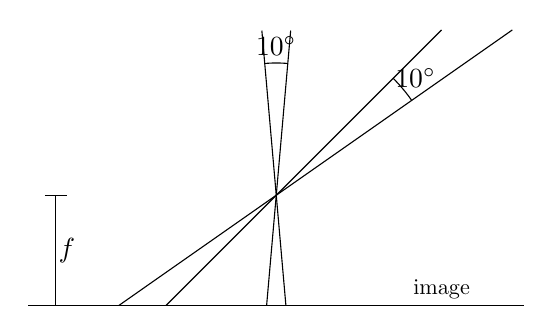
\begin{tikzpicture}[scale=0.7]
        \pgfmathsetmacro{\rvecimg}{2}
        \pgfmathsetmacro{\rvecscene}{3}
        
        \draw[] (0,0,0) -- (95:\rvecscene); \draw[] (0,0,0) -- (85:\rvecscene); 
        \draw[] (0,0,0) -- (-95:\rvecimg); \draw[] (0,0,0) -- (-85:\rvecimg);
        \draw[] (95:0.8*\rvecscene) arc (95:85:0.8*\rvecscene); \draw[] (90:0.9*\rvecscene) node{$10^\circ$};
        
        \draw[] (0,0,0) -- (45:1.414*\rvecscene); \draw[] (0,0,0) -- (35:1.743*\rvecscene); 
        \draw[] (0,0,0) -- (-135:1.414*\rvecimg); \draw[] (0,0,0) -- (-145:1.743*\rvecimg);
        \draw[] (45:\rvecscene) arc (45:35:\rvecscene); \draw[] (40:1.1*\rvecscene) node{$10^\circ$};
        
        \draw[] (-4.5,-\rvecimg,0) -- (4.5,-\rvecimg,0);
        \draw[] (3,-\rvecimg + 0.3,0) node[scale=0.8]{image};
        
        \draw[] (-4,-\rvecimg,0) -- (-4,0,0);
        \draw[] (-4.2,0,0) -- (-3.8,0,0);
        \draw[] (-3.8, -0.5*\rvecimg,0) node{$f$};
        
    \end{tikzpicture}
    \caption{Without lens distortion}
    \label{fig:wide_angle_pinhole_nolens}
    \end{subfigure}
    \begin{subfigure}[b]{0.45\textwidth}
    \centering
    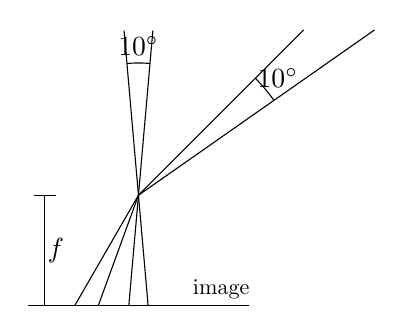
\begin{tikzpicture}[scale=0.7]
        \pgfmathsetmacro{\rvecimg}{2}
        \pgfmathsetmacro{\rvecscene}{3}
        
        \draw[] (0,0,0) -- (95:\rvecscene); \draw[] (0,0,0) -- (85:\rvecscene); 
        \draw[] (0,0,0) -- (-95:\rvecimg); \draw[] (0,0,0) -- (-85:\rvecimg);
        \draw[] (95:0.8*\rvecscene) arc (95:85:0.8*\rvecscene); \draw[] (90:0.9*\rvecscene) node{$10^\circ$};
        
        \draw[] (0,0,0) -- (45:1.414*\rvecscene); \draw[] (0,0,0) -- (35:1.743*\rvecscene); 
        \draw[] (0,0,0) -- (-110:1.064*\rvecimg); \draw[] (0,0,0) -- (-120:1.155*\rvecimg);
        \draw[] (45:\rvecscene) arc (45:35:\rvecscene); \draw[] (40:1.1*\rvecscene) node{$10^\circ$};
        
        \draw[] (-2,-\rvecimg,0) -- (2,-\rvecimg,0);
        \draw[] (1.5,-\rvecimg + 0.3,0) node[scale=0.8]{image};
        
        \draw[] (-1.7,-\rvecimg,0) -- (-1.7,0,0);
        \draw[] (-1.9,0,0) -- (-1.5,0,0);
        \draw[] (-1.5, -0.5*\rvecimg,0) node{$f$};
        
    \end{tikzpicture}
    \caption{With lens distortion}
    \label{fig:wide_angle_pinhole_lens}
    \end{subfigure}
    
    \caption{Amount of image space for different parts of the scene, using a pinhole camera, with and without a camera lens}
    \label{fig:wide_angle_pinhole}
    
\end{figure}

\subsection{Fisheye projection}

The lens distortion of a fisheye lens can be visualized and modeled as projecting the scene onto a sphere. This makes it is easier to describe points in the image plane as spherical coordinates, $P = [X,Y,Z]^\top = [1, \theta,\phi]$. A unit sphere is used to simplify the computations. The sphere is then projected onto a  Figure~\ref{fig:fisheye_spherical_projection} visualizes the image plane of a fisheye lens, with the red lines representing constant $\phi$. The relationship between the image coordinates $p = [x,y]^\top = [r(\phi),\theta]^\top$ and the world coordinates is shown in Equation~\eqref{eq:fisheye_to_image}.

\begin{align}
    r(\phi) &= f \cdot \phi & \theta &= \theta \nonumber \\
    x &= rcos(\theta) & y &= rsin(\theta)
    \label{eq:fisheye_to_image}
\end{align}

\begin{figure}[!htb]
    \centering
    \tdplotsetmaincoords{70}{160}
    \begin{tikzpicture}[tdplot_main_coords, scale = 1.4]
    
    \coordinate (O) at (0,0,0);
    \tdplotsetrotatedcoords{0}{-90}{90}
    \draw[tdplot_rotated_coords, ->] (-0.5,0,0) -- (6,0,0) node[below right]{$X$};
    \draw[tdplot_rotated_coords, ->] (0,-0.5,0) -- (0,2.5,0) node[right]{$Y$};
    \draw[tdplot_rotated_coords, dashed] (0,0,-2.5) -- (0,0,6);
    \draw[tdplot_rotated_coords, ->] (0,0,6) -- (0,0,8) node[below]{$z,Z$};
    
    \tdplotsetcoord{P}{6}{65}{150}
    \draw[] (P) node[above right]{P}; \node at (P){\textbullet};
    \draw[] (O) -- (P);
    
    \tdplotsetcoord{ROTORIG}{7}{90}{180}
    \tdplotsetrotatedcoordsorigin{(ROTORIG)}
    \draw[tdplot_rotated_coords, ->] (180:0.3) arc (180:360:0.3);
    \draw[tdplot_rotated_coords] (0,-0.5,0) node{$\theta$};
    
    \tdplotsetcoord{IMGC}{2}{90}{0}
    \tdplotsetrotatedcoordsorigin{(IMGC)}
    \foreach \x in {-2,-1.5,...,2} {
        \draw[tdplot_rotated_coords] (\x,-2) -- (\x,2);
    }
    \foreach \y in {-2,-1.5,...,2} {
        \draw[tdplot_rotated_coords] (-2,\y) -- (2,\y);
    }
    \foreach \phi in {10,20,...,80} {
        \draw[tdplot_rotated_coords, color=red, opacity = 0.8] (0,0) circle({\phi/45});
    }
    \draw[tdplot_rotated_coords, thick, opacity = 0.8] (0,0) circle(2);
    
    \draw[tdplot_rotated_coords, ->] (-0.5,0,0) -- (4,0,0) node[below right]{$x$};
    \draw[tdplot_rotated_coords, ->] (0,-0.5,0) -- (0,2.5,0) node[right]{$y$};
    \draw[tdplot_rotated_coords, ->] (-2.5,-2,0) -- (2,-2,0) node[below right]{$u$};
    \draw[tdplot_rotated_coords, ->] (-2,-2.2,0) -- (-2,2,0) node[below]{$v$};
    
    \draw[tdplot_rotated_coords] (0,-2.3,0) -- (0,-2.3,2);
    \draw[tdplot_rotated_coords] (0,-2.2,0) -- (0,-2.4,0); \draw[tdplot_rotated_coords] (0,-2.2,2) -- (0,-2.4,2);
    \draw[tdplot_rotated_coords] (0,-2.5,1) node{$f$};
    
    \tdplotsetrotatedcoordsorigin{(O)}
    \draw[thick, tdplot_rotated_coords] (0:2) arc (0:360:2); 
    \foreach \angle in {-90,-95,...,-270} {
        \tdplotsetrotatedcoords{90}{\angle}{0}
        \draw[tdplot_rotated_coords, opacity = 0.7] (0:2) arc (0:180:2);
        
    }
    
    \foreach \angle in {10,20,...,80} {
        \coordinate (TMP) at ({-2*cos(\angle)},0,0);
        \tdplotsetrotatedcoordsorigin{(TMP)}
        \draw[tdplot_rotated_coords, color = red] (0:{2*sin(\angle)}) arc (0:360:{2*sin(\angle)});
    }
    
    \tdplotsetrotatedcoords{90}{-43}{0}
    \draw[tdplot_rotated_coords, ->] (90:5) arc (90:52:5);
    \draw[tdplot_rotated_coords] (70:5.3) node{$\phi$};
    
    \end{tikzpicture}
    
    \caption{Equiangular fisheye lens projection. Focal length exagerated for visual purposes.}
    \label{fig:fisheye_spherical_projection}
\end{figure}

As the spherical projection step makes it easier to handle the world coordinates as spherical coordinates. Using the relationship $X = Rsin(\phi)cos(\theta)$, $Y = Rsin(\phi)sin(\theta)$ and $Z = Rcos(\phi)$ the polar coordinates $R,\theta,\phi$ become:

\begin{equation}
    \begin{aligned}
        R &= X^2 + Y^2 + Z^2 \\
        \theta &= arctan\left(\frac{Y}{X}\right) \\
        \phi &= arccos\left(\frac{Z}{sqrt{X^2 + Y^2 + Z^2}}\right)
    \end{aligned}
    \label{theory_polar_coords}
\end{equation}
\todo[inline]{talk about other fisheye models and distortion effects}

\subsection{Cylindrical projection}

The goal of the cylindrical projection and camera types is to reduce the radial distortion and feature compression, while maintaining the ability to capture images with a horizontal field of view larger than $180^o$. Along the vertical y-axis, the cylindrical projection functions like a pinhole projection, where the mapping is identical to Equation \todo{fix reference and or phrasing}\eqref{eq:pinhole_relation}. For the horizontal axis, the polar coordinate $\theta$ is used, such that the mapping to the image plane becomes:

\begin{subequations}
\begin{equation}
    \theta = arctan\left(\frac{X}{Z}\right)
    \label{eq:cylindrical_theta}
\end{equation}
\begin{equation}
    y = R\frac{Y}{Z}
    \label{eq:cylindrical_y}
\end{equation}
\label{eq:cylindrical}
\end{subequations}

Theoretically this representation removes all vertical radial distortion, however it is still subject to the introduction of distortion through imperfect lenses or image plane alignment. Using the same vertical mapping as the pinhole model, also limits the vertical field of view, causing a top and bottom blind spot.

Cameras using this projection types are not that common, but there are some:...\todo{source}. This projection type is however highly suited to project and stitch pictures taken by a camera rotating around an axis, as is used for the panorama capture function in modern phone cameras\todo{source}.

\subsection{Catadioptric projection}

Using mirrors to reflect the light, early catadioptric lenses could achieve large focal lengths without increasing the physical length of the objective\todo{source}. This made the technology ideal for telescopes and narrow angle imaging. Later, the same principle has developed to include large field of view cameras and panoramic imaging\todo{source}. 

Since the mirror has to be placed within the field of view, the catadioptric lens will always cause a blind spot, and potentially shadows of the mirror mount appearing in the image \todo{source}. To reduce this effect, the mount has to be made more fragile. This may make the cameras unsuited for applications with significant vibrations \todo{source}.

The pixel mapping and field of view is highly dependent on the reflective surface used. Most surfaces will introduce similar radial distortions to the fisheye lens, but there has been developed catadioptric lenses, producing rectilinear projections \todo{source}, however this has to be mounted at a fixed distance from the ground, making them unfit for moving objects. Nayar S. K. made a wide angle, catadioptric lens \todo{source} with a single viewpoint, and proposes further a setup where two of these are mounted back to back to produce a full spherical image. \todo[inline]{Finish the paragraph...}


\subsection{Panomorph projection}

The panomorph lens types are designed around an non-uniform distribution of pixels within the field of view, and is patented by ImmerVision \todo{source/patentsource}. This creates an opportunity to focus on important parts of the field of view, and enhance the resolution in these parts\todo{source}. The lens itself used in these types of cameras resemble the fisheye lens, and share the advantage its advantages over catadioptric lenses\todo{source}. 

Different types of panomorphic lenses has been proposed for different applications. For example in 2010 it was proposed to use a panomorph lens in endoscopy\cite{endoscopypano}. This lens is based on the human eye, and its increased resolution around the center of vision. Other aplications include security cameras\todo{source}, where the outlying areas has been given increased resolution, to counteract the compact representation provided by normal fisheye cameras.

Since the pixel density varies within the field of view, the lens is more difficult to construct as well as model. Fortunately, different types of distortion control are available today\todo{source}, as well as calibration tools. Depending on the amount of distortion, the solution may be hard to simulate in real time. Especially with reduced computing power \todo{source}.

\subsection{Merging multiple camera views}

\section{Computer graphics}

Our eyes and cameras capture the 3D world from light hitting photosensitive elements. An object directly or partly behind another object will therefore be hidden in the picture, unless captured by a reflection. In addition to this, shadows, colors and lighting of objects in the scene are all based on how the light rays bounce around in the room, and eventually hit the camera lens. In computer graphics, there is no inherent concept of light. This means that all the effects that are based around light must be estimated or simulated. Since calculating light and shadow effects are quite expensive computationally, it is not uncommon to add shadow elements directly to the object texture, in order to optimize the for speed.

There are two main approaches: One approach is Ray tracing, which simulates light rays as they travel in straight lines from the camera center, through a pixel. When a ray hits an object, the ray is split in two, creating a shadow ray following the same trajectory through the object, and a reflection ray following the reflection trajectory. Ultimately these rays will find a light source, leave the scene. Usually the rays are limited to a number of bounces, to save some computation. This technique is incredibly powerful, and is used heavily in CGI effects for film making. However, the amount of computation necessary makes it hard to incorporate this in real-time applications.

The other approach is often referred to as rasterization, and is the one used most in real-time applications. Rasterization is a actually only a step in a larger pipeline of graphics computations, and comes after the clipping and culling stages, deciding which parts of each object that are visible. The task of rasterization is choosing which visible object to show in each pixel. The main advantage Razterization has is it's short computation time and ability to be parallelized. The downside is that it captures much less information about the lighting, providing the shader much less information for the final coloring.

\subsection{Graphics projection}

One of the main difficulties in graphics programming is deciding which objects are visible. In simple terms, this consists of two tasks: Clipping, or deciding what os outside the FoV, and Culling, which decides which objects in the line of sight, that are cosest to the viewer. In order to simplify computations, the visible scene is projected into a cube of a known size. This is usually the cube consisting of the points $x, y, z \in [-1,1]$, or $x,y \in [-1,1], z \in [0,1]$. however, both the cube size and the placement may differ from renderer to renderer. This means that the term projection in computer graphics, refer to a tranformation from $\mathbb{R}^3 \rightarrow \mathbb{R}^3$ while camera projections refer to a direct transformation to the image plane, from $\mathbb{R}^3 \rightarrow \mathbb{R}^2$.

There are two main projection types used: orthographic and perspective. Orthographic projection is specially made to keep the scale of the object independent on how far away it is from the camera. This makes it ideal for schematics and other computer aided design, where the size of the drawing must be proportional to the real size of the object. The other type is perspective projection, and will be the one which is relevant for this project.

\subsection{Perspective projection}

As seen in Figure~\ref{fig:perspective_projection}, perspective projection has a lot in common with the pinhole projection, as the scaling of objets seen in Equation~\eqref{eq:pinhole_tan_relation} also holds for perspective projection, preserving the depth of the picture. The difference comes from the addition of a near and a far clipping plane. Which limits the visible scene to a confined space, and limits the amount of computations needed. Figure~\ref{fig:perspective_proj_yz} shows the yz-view of a perspective projection. Here $a^*$ and $b^*$ are references to where point $a$ and $b$ will show in the projection, $\Theta$ is the FoV and $d_n$, $d_f$ are the distance to the near and far clipping plane.

\begin{figure}[!htb]
    \centering
        \begin{tikzpicture}[scale=1.0]
            \coordinate (O) at (0,0,0);
            \coordinate (OL) at (-7,0,0);
            \coordinate (OH) at (4,0,0);
        
            \draw[dashed, ->] (-7.3,0) -- (-1,0) node[below right]{$Z$};
            \draw[->] (-7,1.5) -- (-7,-1.5) node[above left]{$Y$};
            
            \draw[->] (1,0) -- (7.3,0) node[below right]{$z$};
            \draw[->] (4,3) -- (4,-3) node[right]{$y$};
            
            \tdplotsetrotatedcoordsorigin{(OH)}
            \draw[tdplot_rotated_coords] (-1.5,-1.5) -- (-1.5,1.5) node{\textbullet} node[below right]{$a^*$} -- (1.5,1.5) node{\textbullet} node[below right]{$b^*$}-- (1.5,-1.5) -- cycle;
            
            \draw[tdplot_rotated_coords] (1.5,0) node[below right]{\scriptsize $1$};
            \draw[tdplot_rotated_coords] (0,-1.5) node[below right]{\scriptsize $1$};
            \draw[tdplot_rotated_coords] (0,1.5) node[above right]{\scriptsize $-1$};
            \draw[tdplot_rotated_coords] (-1.5,0) node[below left]{\scriptsize $-1$};
        
            \tdplotsetrotatedcoordsorigin{(OL)}
            \draw[tdplot_rotated_coords, ->] (0,0) -- (15:5.5);
            \draw[tdplot_rotated_coords, ->] (0,0) -- (-15:5.5);
            
            \draw[tdplot_rotated_coords] (1.5, {1.5*tan(-15)}) -- (1.5,{1.5*tan(15)});
            \draw[tdplot_rotated_coords] (1.5, {1.5*tan(-15)}) -- (1.5,{1.5*tan(15)});
            
            \draw[tdplot_rotated_coords] (4, {4*tan(-15)}) -- (4,{4*tan(15)});
            \draw[tdplot_rotated_coords] (4, {4*tan(-15)}) -- (4,{4*tan(15)});
            
            \draw[tdplot_rotated_coords] (15:2) arc (15:-15:2);
            \draw[tdplot_rotated_coords] (2.2,0.2) node{$\Theta$};
            
            \draw[tdplot_rotated_coords] (1.5,{1.5*tan(15)}) node{\textbullet} node[above left]{$a$};
            \draw[tdplot_rotated_coords] (4,{4*tan(15)}) node{\textbullet} node[above left]{$b$};
            
            \draw[tdplot_rotated_coords] (0,-1.8) -- node[midway, above]{$d_n$} ++(1.5,0);
            \draw[tdplot_rotated_coords] (0,-1.9) -- (0,-1.7); \draw[tdplot_rotated_coords] (1.5,-1.9) -- (1.5,-1.7);
            \draw[tdplot_rotated_coords] (0,-2.2) -- node[midway, above]{$d_f$} ++(4,0);
            \draw[tdplot_rotated_coords] (0,-2.3) -- (0,-2.1); \draw[tdplot_rotated_coords] (4,-2.3) -- (4,-2.1);
            
        \end{tikzpicture}
    \caption{yz-view of perspective projection, with $a^*,b^*$ being the projected version of $a,b$}
    \label{fig:perspective_proj_yz}
\end{figure}

The height of the near clipping plane will always be $2$. This means that the vertical FoV $\Theta$ is directly linked to the distance $d_n$.  Using this information, as well as the tangential relationship from Equation~\eqref{eq:pinhole_tan_relation}, the projection of $Y$ can be deduced, as shown in Equation~\eqref{eq:perspective_y}. To describe the projection of $X$ we may use the aspect ratio to form a relationship between the horizontal and vertical FoV. Equation \eqref{eq:perspective_fov_relation} shows this, with the horizontal FoV denoted as $\Theta_H$. The projection of $X$ is shown in Equation~\eqref{eq:perspective_x}.

\begin{equation}
    Zy^* = \frac{Y}{tan\left(\frac{\Theta}{2}\right)} = Z \Rightarrow y^* = \frac{1}{tan\left(\frac{\Theta}{2}\right)}\frac{Y}{Z}
    \label{eq:perspective_y}
\end{equation}

\begin{subequations}
\begin{equation}
    tan\left(\frac{\Theta_H}{2}\right) = \frac{W}{H}tan\left(\frac{\Theta}{2}\right)
    \label{eq:perspective_fov_relation}
\end{equation}
\begin{equation}
    x^* = \frac{\rho}{tan\left(\frac{\Theta}{2}\right)}\frac{X}{Z} \quad , for \quad \rho = \frac{Width}{Height}
    \label{eq:perspective_x}
\end{equation}
\label{eq:perspective_x_fovrel}
\end{subequations}


\begin{figure}[!htb]
    \centering
    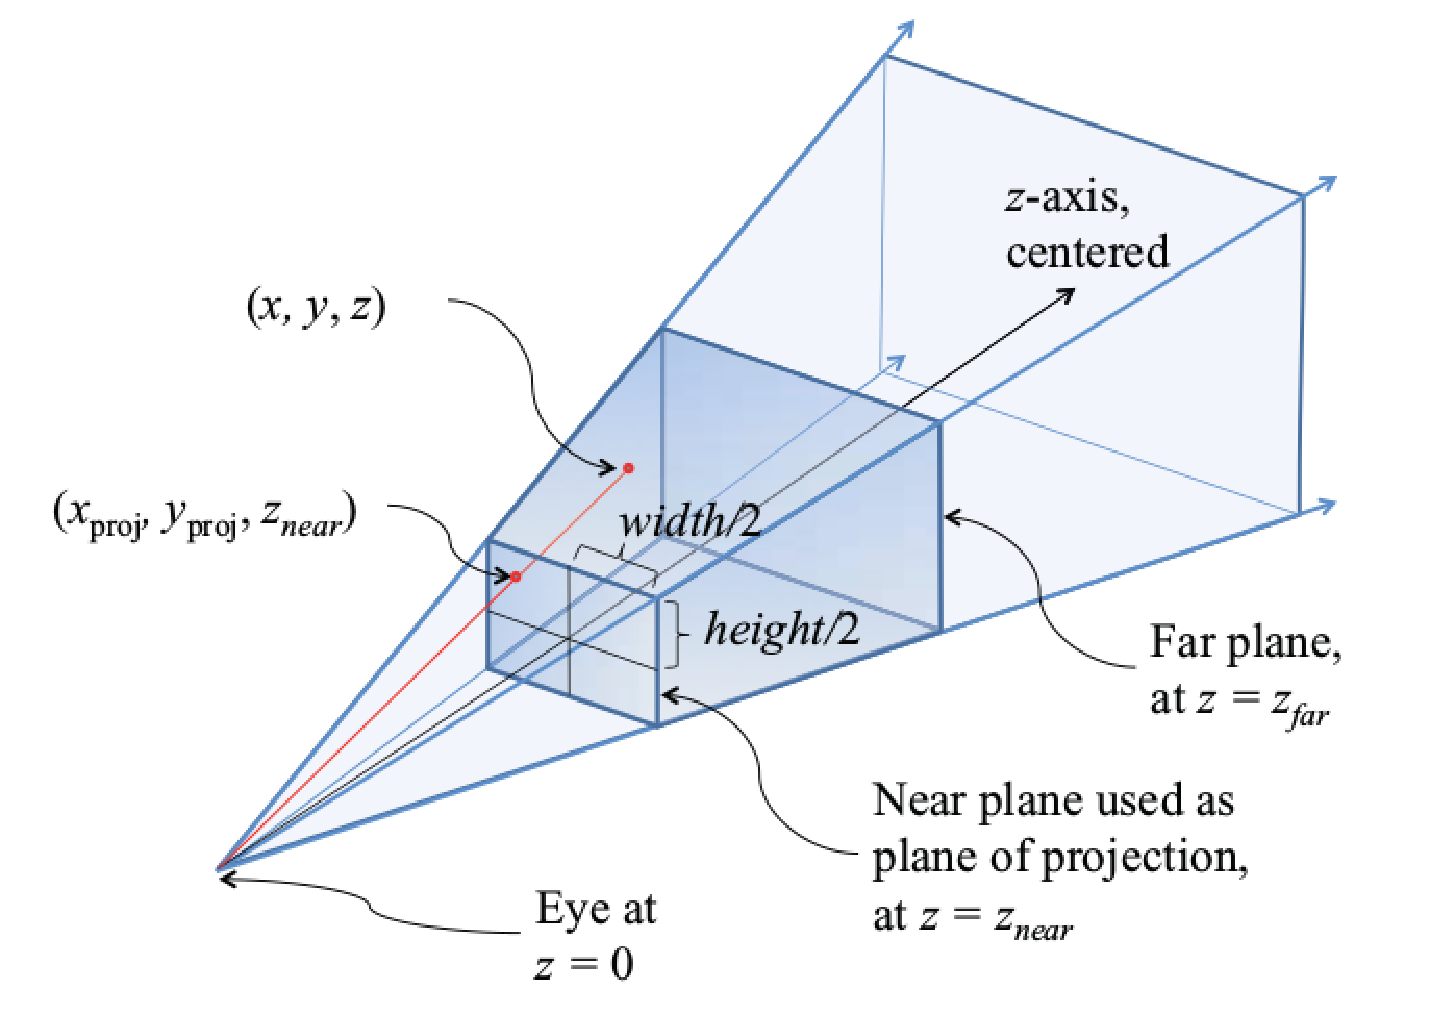
\includegraphics[width=0.6\textwidth]{perspective_projection}
    \caption{Perspective projection with combined projection plane and near clipping plane}
    \label{fig:perspective_projection}
\end{figure}

While the projection of $X$ and $Y$ more or less are equal for most renderer implementations, the projection of $Z$ is highly dependent on the chosen target cube, as well as the orientation of the Z-axis. Using the homogenous scene coordinates $P = [X,Y,Z,1]^\top$ and $p* = [x,y,z,w]^\top$ the transformation can be written as shown in Equation~\eqref{eq:perspective_projmat_temp}. Here $w = Z$ to scale $X$ and $Y$, and needs to be taken into account when calculating the $Z$ projection. Since both clipping planes have the z-axis as a plane normal in both the original scene, as well as the projected cube, $z$ will be independent on $X$ and $Y$ simplifying the computation to the set of two equations shown in Equation~\eqref{eq:perspective_zeqs}.


\begin{align}
    p^* &= \begin{bmatrix}
        x \\ y \\ z \\ w
    \end{bmatrix} = \begin{bmatrix}
        \frac{\rho}{tan\left(\frac{\Theta}{2}\right)}& 0 & 0 & 0 \\
        0 & \frac{1}{tan\left(\frac{\Theta}{2}\right)}& 0 & 0 \\
        0 & 0 & A & B \\
        0 & 0 & 1 & 0
    \end{bmatrix} \begin{bmatrix}
        X \\ Y \\ Z \\ 1
    \end{bmatrix} & p &= \frac{1}{w}p^* \label{eq:perspective_projmat_temp}
\end{align}


\begin{equation}
    \begin{aligned}
        zd_n &= Ad_n + B &, for \quad Z &= d_n \\
        zd_f &= Ad_f + B &, for \quad Z &= d_f
    \end{aligned}
    \label{eq:perspective_zeqs}
\end{equation}



% Solving this we get;

% \begin{align}
%     A &= \frac{n}{n-f} & B &= -\frac{nf}{n-f}
% \end{align}

% resulting in the complete perspective projection shown in Equation~\eqref{eq:perspective_projmat_full}.

% \begin{align}
%     p^* &= \begin{bmatrix}
%         x \\ y \\ z \\ w
%     \end{bmatrix} = \begin{bmatrix}
%         \frac{\rho}{tan\left(\frac{\Theta}{2}\right)}& 0 & 0 & 0 \\
%         0 & \frac{1}{tan\left(\frac{\Theta}{2}\right)}& 0 & 0 \\
%         0 & 0 & \frac{n}{n-f} & -\frac{nf}{n-f} \\
%         0 & 0 & 1 & 0
%     \end{bmatrix} \begin{bmatrix}
%         X \\ Y \\ Z \\ 1
%     \end{bmatrix} & p &= \frac{1}{w}p^*
%     \label{eq:perspective_projmat_full}
% \end{align}

% \subsection{Ray Tracing}

% Ray tracing techniques have existed as a fully developed technique since 1986 \cite{raytraceblog}. Today, Ray tracing is highly used in film making for CGI, which is Computer-generated imagery to be applied on its own, or in the same frame as actual camera footage. The inherent ability ray tracing has to mimic real world light, enables the algorithms to produce very realistic images. The downside is that tracing light rays, all their reflections, refractions and shadows they cast, is really computationally expensive.

% Since 1986 much research has gone into improving the rendering time of these images. \cite{wald2009state} summarizes many of these, but also shows the conflicts between ray tracing approaches for video games, and approaches for movie making. The article states that the movie making approach is centered around making data structures for efficient computation, while more or less ignoring the building time of these structures. This can be backed up by Section 3 of \cite{carsmovie}, where the main focus is shown to be memory management and quality. In real time applications however, these data structures needs to be built and rebuilt, in addition to the computation, in real time. 

% Nvidia recently developed their RTX-series of graphics cards \cite{raytraceblog}, promising to revolutionize the ways shadows, reflections and lighting are shown in real-time image processing, with the use of ray tracing. Based on their launch event presentation \cite{NvidiaConference}, this will be realized by; the integration of ray tracing cores, a locally developed ray tracing acceleration algorithm and deep learning. The ray tracing cores are are specialized processing units, designed to parallelize ray tracing calculations, while the ray tracing acceleration refers to a search algorithm for finding intersections between light rays and objects. Lastly the deep learning portion uses a previously trained deep learning network, made specifically to upscale and fill in the gaps of lower quality images, with the goal of reducing the amount of rays needed to be calculated, as well as to perform anti-aliasing tasks.

\cleardoublepage